\chapter{Quiz Pertemuan V}


\section{Permasalahan}
\begin{permasalahan}{Awal-Tengah-Akhir}\\
\label{prob:Alfa-Mid-Omega}
	Diberikan sebuah kata yang terdiri dari alfabet, dapatkah kamu menentukan huruf awal, tengah dan terakhir ? \\\\
	\textbf{Masukan}\\
	Sebuah kata bertipe data string dengan panjang kata pasti ganjil\\
	\textbf{Keluaran}\\
	(huruf awal) (huruf tengah) (huruf terakhir)\\
	\begin{center}
	\textbf{Test Case 1}\\
	\end{center}
	\textbf{Masukan}\\
	algoritma\\
	\textbf{Keluaran}\\
	a r a \\
	\begin{center}
	\textbf{Test Case 2}\\
	\end{center}
	\textbf{Masukan}\\
	machine\\
	\textbf{Keluaran}\\
	m h e\\
	\begin{center}
	\textbf{Test Case 3}\\
	\end{center}
	\textbf{Masukan}\\
	ada\\
	\textbf{Keluaran}\\
	a d a\\
\end{permasalahan}


\newpage
\begin{permasalahan}{Jam-Menit-Detik}\\
\label{prob:Jam-Menit-Detik}
	Diberikan dua informasi waktu dalam sekian jam, sekian menit dan sekian detik. Hitung selisih dari kedua waktu dalam  format yang paling baik tersebut !\\\\
	\textbf{Masukan}\\
	Dua buah string dengan format ``jam menit detik``. Masukkan dapat mengandung kombinasi jam, menit, detik yang tidak dalam format paling tepat \\
	\textbf{Keluaran}\\
	Sebuah string dengan format ``jam menit detik`` \textbf{dengan format yang yang paling tepat dan sederhana}\\
	\begin{center}
	\textbf{Test Case 1}\\
	\end{center}
	\textbf{Masukan}\\
	2 0 0\\
	1 0 0\\
	\textbf{Keluaran}\\
	1 0 0\\
	\begin{center}
	\textbf{Test Case 2}\\
	\end{center}
	\textbf{Masukan}\\
	1 0 0\\
	2 0 0\\
	\textbf{Keluaran}\\
	1 0 0\\
	\begin{center}
	\textbf{Test Case 3}\\
	\end{center}
	\textbf{Masukan}\\
	0 0 3600\\
	1 120 0 \\
	\textbf{Keluaran}\\
	2 0 0\\
	\begin{center}
	\textbf{Test Case 4}\\
	\end{center}
	\textbf{Masukan}\\
	3 1 1\\
	1 59 40 \\
	\textbf{Keluaran}\\
	1 1 21\\
	\begin{center}
	\textbf{Test Case 5}\\
	\end{center}
	\textbf{Masukan}\\
	1 59 40 \\
	3 1 1   \\
	\textbf{Keluaran}\\
	1 1 21\\
\end{permasalahan}

\newpage
\begin{permasalahan}{Pembilang Per Penyebut ? Bulat !}\\
\label{prob:PembilangPerPenyebut}
	Anda diminta untuk mencetak pecahan jika diberikan informasi inisialisasi pembilang dan penyebut, penambahan barisan per langkah dan banyak barisan. \\
	Pembilang dan Penyebut yang menghasilkan bilangan bulat, harus dicetak dalam bentuk bilangan bulat !
	\textbf{Masukan}\\
	(Pembilang awal) (Penyebut awal) (step Pembilang) (step Penyebut) (banyak barisan) \\
	Semua masukkan dalam bentuk bilangan bulat positif\\
	\textbf{Keluaran}\\
	Barisan suku ke 1 sampai suku ke-(banyak barisan) yang dipisahkan per baris / (new-line)\\
	\begin{center}
	\textbf{Test Case 1}\\
	\end{center}
	\textbf{Masukan}\\
	1 2 0 3 5\\
	\textbf{Keluaran}\\
	1/2\\
	1/5\\
	1/8\\
	1/11\\
	1/14\\
	\begin{center}
	\textbf{Test Case 2}\\
	\end{center}
	\textbf{Masukan}\\
	1 1 1 1 5\\
	\textbf{Keluaran}\\
	1\\
	1\\
	1\\
	1\\
	1\\
\end{permasalahan}



\newpage
\begin{permasalahan}{PolaloP}\\
\label{prob:PembilangPerPenyebut}
	Diberikan ukuran dari pola cetaklah pola yang akan ditunjukkan pada keluaran berikut ! \\
	\textbf{Masukan}\\
	Sebuah bilangan bulat positif yang menyatakan ukuran\\
	\textbf{Keluaran}\\
	Pola seperti yang ditunjukkan pada keluaran\\
	\begin{center}
	\textbf{Test Case 1}\\
	\end{center}
	\textbf{Masukan}\\
	1\\
	\textbf{Keluaran}\\
		\begin{figure}[h!]
		
\includegraphics{fig/Bintang/1.png}	
		\end{figure}

	\begin{center}
	\textbf{Test Case 2}\\
	\end{center}
	\textbf{Masukan}\\
	2\\
	\textbf{Keluaran}
		\begin{figure}[h!]
		
\includegraphics{fig/Bintang/2.png}	
		\end{figure}

	\begin{center}
	\textbf{Test Case 3}\\
	\end{center}
	\textbf{Masukan}\\
	3\\
	\textbf{Keluaran}\\
		\begin{figure}[h!]
		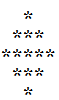
\includegraphics{fig/Bintang/3.png}	
		\end{figure}
	\begin{center}
	\textbf{Test Case 4}\\
	\end{center}
	\textbf{Masukan}\\
	4\\
	\textbf{Keluaran}\\
		\begin{figure}[h!]
		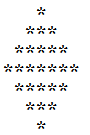
\includegraphics{fig/Bintang/4.png}	
		\end{figure}
		\begin{center}
	\textbf{Test Case 5}\\
	\end{center}
	\textbf{Masukan}\\
	5\\
	\textbf{Keluaran}\\
		\begin{figure}[h!]
		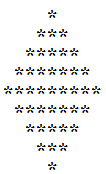
\includegraphics{fig/Bintang/5.png}	
		\end{figure}
\end{permasalahan}
